\documentclass[11pt,a4j,titlepage]{jsarticle}
\usepackage[dvipdfmx]{graphicx}
\usepackage{amsmath, amssymb}
\usepackage{float}
\usepackage{multirow}
\usepackage{url}
\usepackage{subcaption}
\usepackage{tabularx}
\usepackage{listings, jlisting}
\usepackage{here}
\lstset{
basicstyle={\small\ttfamily},
identifierstyle={\small},
keywordstyle={\small\bfseries},
ndkeywordstyle={\small},
stringstyle={\small\ttfamily},
frame={tb},
breaklines=true,
columns=[l]{fullflexible},
numbers=left,
xrightmargin=0zw,
xleftmargin=3zw,
numberstyle={\scriptsize},
stepnumber=1,
numbersep=1zw,
lineskip=-0.5ex
}
\begin{document}
\title{ネットワーク実験レポート課題}
\author{学正番号:09B21601 氏名:西澤陽}
\date{提出日2024/1/22}
\maketitle
\section{プログラムの処理方針と作成方針}
本実験で作成プログラムはサーバー側とクライアント側でデータの通信を行うプログラムである.
\subsection{作成方針}
本プログラムではサーバー側とクライアント側を分けて別々に作成する.初めにクライアント側について作成する.目標はWebサーバーに対して,HHTPを用いて接続し,Webコンテンツを取得することである.

クライアント側が完成したら,サーバー側を作成する.目標は既に作成したクライアントと1度に一つの通信可能なサーバーを作成することである.

サーバーとクライアントが完成したら,名簿管理プログラムをサーバー,クライアント通信へ拡張する.通信の概要はサーバー側で名簿プログラムを動かし,クライアントから送られてくるコマンドをサーバー側で実行し,結果をクライアントに返すシステムである.
\subsection{処理方針}\label{shorihou}
本プログラムの処理方針について述べる.初めにクライアントで通信相手の情報を取得し,情報からソケットを作成する.
その間にサーバー側では待ち受けソケットを作成し.ソケットを待ち受け設定にする.サーバー側で待ち受けを開始する.その後,クライアントがTCPコネクション確立を試みる.それに対して,サーバーはコネクションを受け入れ,クライアントとサーバー同士でデータの送受信を行う.最後に共にデータ通信ソケットを終了させ,通信が終了する.

\section{プログラム処理の説明}
本章ではプログラム処理をソートコードと併せて解説する.
クライアントとサーバーの順番で解説する.
\subsection{クライアント}
始めに通信相手について調べる処理を行う.このとき用いるのがgetaddrinfo関数である.初めに最低限の設定をした構造体addrinfo hintsを作成する.構造体のメンバを本実験では以下のように設定した.
\begin{lstlisting}[caption=addrinfo hintsの設定,label=]
  memset(&hints,0,sizeof(hints));
  hints.ai_socktype = SOCK_STREAM;
  hints.ai_family = AF_INET;
  if(getaddrinfo(argv[1],argv[3],&hints,&res) !=0){
        printf("error:getaddrinfoargv[0]= %s\n",argv[1]);
    }
\end{lstlisting}
hintsを0埋めし,2行目でソケットタイプをTCPに設定する.3行目で受け入れるプロトコルファミリーをIPv4に設定している.
以上の設定と,通信相手のIPアドレスもしくはドメイン名,接続ポート番号を決定したgetaddrinfo関数で通信相手の情報を取得する.取得した情報はresに格納され,以降はこれを使う.

次は通信を確立する工程について説明する.socket関数にresに格納された通信の前提となる情報を与え,ソケットを作成する.通信を確立するためにconnect関数にソケット,通信相手のIPアドレス等を与える.通信を確立しようとした時,サーバー側で待ち受け状態であると接続要求が受け入れられ通信が始まる.

通信が始まると,クライアントでは標準入力で名簿管理プログラムを動かすためのコマンドを受け付ける.コマンドを0埋めしたバッファsend\_mesに格納し,サーバー側に送信する.標準入力から送信までのプログラムを以下に示す.
\begin{lstlisting}[caption=標準入力とその送信,label=]
  memset(send_mes,0,sizeof(send_mes));
  n = read(0,send_mes,256);
  if(n==-1||n==0){
      printf("ファイルの読み込みエラー\nat:inToOut");
      exit(0);
  }
  ~省略~
  if(send(s,send_mes,BUF_SIZE,0)==-1)
  {
          fprintf(stderr,"sendERROR\n");
          return 0;
  }
\end{lstlisting}
memset関数でsend\_mesを0埋めしている.標準入力をread関数で行いsend\_mesに結果を格納している.read関数のエラー処理は3から6行目で行っている.7行目でsend関数にソケット,バッファとそのサイズを渡しサーバー側へバッファ内容を送信している.send関数にてエラーが起きると,返り値が-1となるため以降の行でエラー処理をしている.
送信が完了するとサーバー側から応答があり,recv関数で受信し,myprintで表示する.ソケットの作成から,受信内容を表示までの一連の処理をクライアントが終了するまで繰り返す.
省略箇所は\%Qが入力されたときの記述である.

なお\%Qが入力された場合のみクライアントを終了させる仕様があるため,別にプログラム記述した.
\begin{lstlisting}[caption=\%Qが入力された時の処理,label=]
  int next_procec(char *input){
    //printf("%d:next_procec\n",strlen(input));
    if (strcmp(input, "%Q") == 0) {
        return 0;
    }else if(input[0]=='%'){
        return 1;
    } else {
        printf("一致する文字列がありません\n");
        return -1;
    }
}
  //%Qの処理
  if(next_procec(send_mes)==0)
  {
      printf("クライアント終了\n");
      if(send(s,err_mes,BUF_SIZE,0)==-1)
      {
              fprintf(stderr,"sendERROR\n");
              return 0;
      }
      recv(s,buf,BUF_SIZE,0);
      close(s);
      break;
  }
\end{lstlisting}
next\_procec関数はsend\_mesの中身が\%Qか確認する関数である.\%Qなら0を返し,13から24行目の処理を行う.ここではsend関数でerr\_mesを送信する.err\_mesには"NON"という文字列が格納されており,特に文字列に意味はない.クライアントの送信に対する応答を受け取ったのち22行目のclose関数でソケットを削除している.
\subsection{サーバー}\label{sec:ser}
次にサーバーでの処理の説明をする.
初めにsocket関数でソケットを作成する.IPプロトコルはIPv4,トランスポートプロトコルはTCPのため引数は以下のように設定した.
\begin{lstlisting}[caption=ソケットの作成(サーバー側),label=]
  s_s=socket(AF_INET, SOCK_STREAM, 0);
  if(s_s==-1){
      fprintf(stderr,"socket\n");
      return -1;
  }
\end{lstlisting}

ここでTCP/IP用のsockaddr構造体のメンバを設定する.メンバの値は以下のように設定した.
\begin{lstlisting}[caption=sockaddr構造体のメンバ設定,label=]
  sa.sin_family = AF_INET;
  sa.sin_addr.s_addr = htonl(INADDR_ANY);
  sa.sin_port = htons((uint)atoi("61002"));
\end{lstlisting}
sockaddr構造体saのメンバの設定について説明する.1行目ではIPプロトコルをIPv4に,2行目ではIPアドレスによる接続を制限に関する設定をしている.上記の設定では,IPアドレスによる制限を設けていない.3行目は待ち受けポート番号を設定している.

ソケットの待ち受け設定とソケットでサーバーとしての待ち受け設定を開始する.待ち受け設定はbind関数,待ち受け設定の開始はlisten関数を用いる.以下に2つの関数を使用したプログラムを示す.
\begin{lstlisting}[caption=ソケットの待ち受け設定とソケットでサーバーとしての待ち受け設定を開始,label=]
  if(bind(s_s, (struct sockaddr*)&sa, sizeof(sa)) == -1)
  {
      fprintf(stderr,"bindERROR (%s)\n",strerror(errno));
      return -1;
  }
  printf("bind is done\n");

  if(listen(s_s,5) == -1)
  {
      fprintf(stderr,"listenERROR\n");
      return -1;
  }
  printf("listen is done\n");
\end{lstlisting}
1行目ではソケットの待ち受け設定をbind関数で行っている.
第1引数に待ち受け用ソケットを渡し,設定として第2引数にsockaddr構造体を与えている.sockaddrの終わりがわかるように,saのサイズを渡している.bind関数のエラー処理は1から5行目で行っている.8行目では待ち受け設定の開始をlisten関数で行っている.サーバーとして待ち受けを開始したソケットを第1引数に渡し,一度に通信できる相手の最大数を第2引数で指定している.本プログラムでは5人と最大通信できる.

この後の処理は,クライアントと連続して通信をするために繰り返し処理を行う.
初めに,listen状態中にソケットへきた接続要求を受け取り,データ通信用のソケットを作成する.
\begin{lstlisting}[caption=データ通信用のソケットを作成,label=]
  len = sizeof(ca);
  news = accept(s_s,(struct sockaddr*)&ca,&len);
  if(news==-1){
      err_num=errno;
      fprintf(stderr,"acceptingERROR (%s)\n",strerror(err_num));
      return 0;
  }
  printf("Connection accepted from %s:%d\n", inet_ntoa(ca.sin_addr), ntohs(ca.sin_port));
\end{lstlisting}
2行目のaccept関数でデータ通信用のソケットを作成している.accept関数の返り値が通信用のソケットとなる.本プログラムでは,通信用のソケットはnewsとした.また第2引数は接続相手に関する情報を取得するためsockaddr構造体caを渡した.次の処理はクライアントからのメッセージの受信と,それに対する応答の送信である.以下にプログラムを示す.
\begin{lstlisting}[caption=クライアントからのメッセージの受信と,それに対する応答の送信,label=]
  if(recv(news,buf,BUF_SIZE,0) == -1){
    fprintf(stderr,"recvERROR\n");
  }
  myprint(buf);
  printf("receive is done\n");
  if(strcmp(buf,"NON")!=0)isParse=parse_input(buf);

  if(send(news,sending,BUF_SIZE,0)==-1)
  {
          fprintf(stderr,"sendERROR (%s)\n",strerror(errno));
  }
  printf("sending is done\n");
  printf("~~~~~~~~~~~~~~~~~~~~~~~~~ALL DONE~~~~~~~~~~~~~~~~~~~~~~~~\n");
  close(news);

\end{lstlisting}
1行目のrecv関数で通信相手から送信されてくるメッセージをbufに格納する.1~3行目はrecv関数に関するエラー処理である.6行目でstrcmp関数で受信メッセージがNONでない場合,parse\_input関数にbufを渡し,名簿プログラムを起動する.名簿管理プログラムでの出力結果はグローバル変数senndingに格納されている.通信用ソケットをsend関数に渡し,名簿管理プログラムの出力結果を格納したsendingをクライアントに送る.その処理が8行目で,以降11行目までがエラー処理処理である.受信と送信が完了したら,通信用ソケットを破棄する.サーバー側はクライアントからの通信を待ち続けるため,再びクライアントからの通信要求をacccept関数で待ち一連の処理を繰り返す.
\section{プログラムの使用方法と使用例}
本章ではプログラムの使用方法と使用例を述べる.
表\ref{tab:howtouse}に使用方法を示す.
\begin{table}[]
  \centering
  \caption{プログラムの使用方法}
  \label{tab:howtouse}
  \begin{tabular}{|c|l|}
  \hline
  コマンド     & 動作            \\ \hline
  \%Q      & 終了            \\ \hline
  \%C      & 登録件数の表示       \\ \hline
  \%P n    & 先頭からn件表示      \\ \hline
  \%R file & fileから読み込み    \\ \hline
  \%W file & fileへ書き出し     \\ \hline
  \%F word & wordを検索       \\ \hline
  \%S n    & データをn番目の項数で整列 \\ \hline
  \end{tabular}
  \end{table}

表\ref{tab:howtouse}の主に使うコマンド(\%Q,\%C,\%P,\%R)動作例を節に分けて示す.
\subsection{サーバーとクライアントの起動}
始めにサーバーとクライアントの起動について説明する.初めにサーバーを起動したときの動作を図\ref{fig:ser_sta}に,クライアントを起動したときの動作を図\ref{fig:cli_sta}に示す.
\begin{figure}[h]
\centering
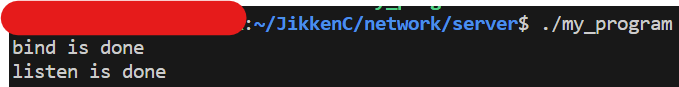
\includegraphics[width=10cm]{pics/server_start.png}
\caption{サーバーを起動したときの動作}
\label{fig:ser_sta}\vspace{0zh}
\end{figure}
\begin{figure}[h]
\centering

\includegraphics[width=10cm]{pics/client_start.png}
\caption{クライアントを起動したときの動作}
\label{fig:cli_sta}\vspace{0zh}
\end{figure}

サーバーではプログラムを開始するのみである.図\ref{fig:ser_sta}より,\ref{sec:ser}章で説明したbindとlisten関数の処理が完了している.対して,クライアントを開始する場合はコマンドライン引数の第1引数に接続先IPアドレス(今回localhost),第3引数に接続先ポート番号を指定する.クライアントを開始した時点で,既にサーバーは接続要求を待っているため,通信が開始する.通信が開始したときのサーバーの動作を図\ref{fig:ser_conesta}に示す.
\begin{figure}[h]
\centering
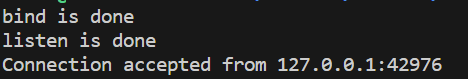
\includegraphics[width=10cm]{pics/server_connected.png}
\caption{通信が開始したときのサーバーの動作}
\label{fig:ser_conesta}\vspace{0zh}
\end{figure}

図\ref{fig:cli_sta}と\ref{fig:ser_conesta}の状態を確認したら,表\ref{tab:howtouse}記載のコマンドをクライアント側にて入力する.
\subsection{\%Qの動作}
クライアントで\%Qを入力したときの動作を図\ref{fig:Q_cli},サーバーで\%Qを入力したときの動作を図\ref{fig:Q_ser}に示す.
\begin{figure}[]
\centering
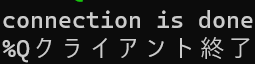
\includegraphics[width=10cm]{pics/Q_client.png}
\caption{クライアントで\%Qを入力したときの動作}
\label{fig:Q_cli}\vspace{0zh}
\end{figure}
\begin{figure}[tbp]
\centering
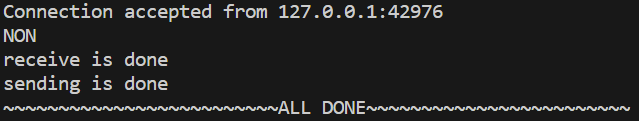
\includegraphics[width=10cm]{pics/Q_server.png}
\caption{サーバーで\%Qを入力したときの動作}
\label{fig:Q_ser}\vspace{0zh}
\end{figure}

図\ref{fig:Q_cli}より,\%Qをクライアントで入力すると,クライアントプログラムが終了していることがわかる.次に図\ref{fig:Q_ser}より,\%Qをクライアントから受け取ると,受け取ったバッファが"NON"になっており,空の文字列を送信し通信用ソケットを破棄している.
\subsection{\%Cの動作}
\%Cは登録件数を表示するコマンドである.プロフィールを登録していない状態で\%Cを入力したときの動作を図\ref{fig:c0},3件登録してから\%Cを入力したときの動作を図\ref{fig:cn}に示す.
\begin{figure}[h]
\centering
\includegraphics[width=10cm]{pics/C0.png}
\caption{プロフィールを登録していない状態で\%Cを入力したときの動作}
\label{fig:c0}\vspace{0zh}
\end{figure}
\begin{figure}[h]
\centering
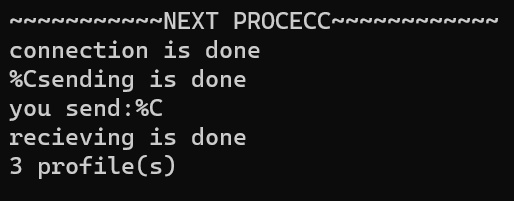
\includegraphics[width=10cm]{pics/C3.png}
\caption{3件登録してから\%Cを入力したときの動作}
\label{fig:cn}\vspace{0zh}
\end{figure}

何も登録していない状態で\%Cを入力すると0 profilesと表示され,何も登録されていないことがわかる.対して,3件登録した後に\%Cを入力すると3 profilesと3件登録されていることがわかる.
\subsection{\%P}
\%Pは登録してあるプロフィールを表示するコマンドである.\%P 2で2件プロフィールを表示したときの動作を図\ref{fig:p2},\%P 0で登録してある全件を表示した時の動作を図\ref{fig:p0}に示す.
\begin{figure}[h]
\centering
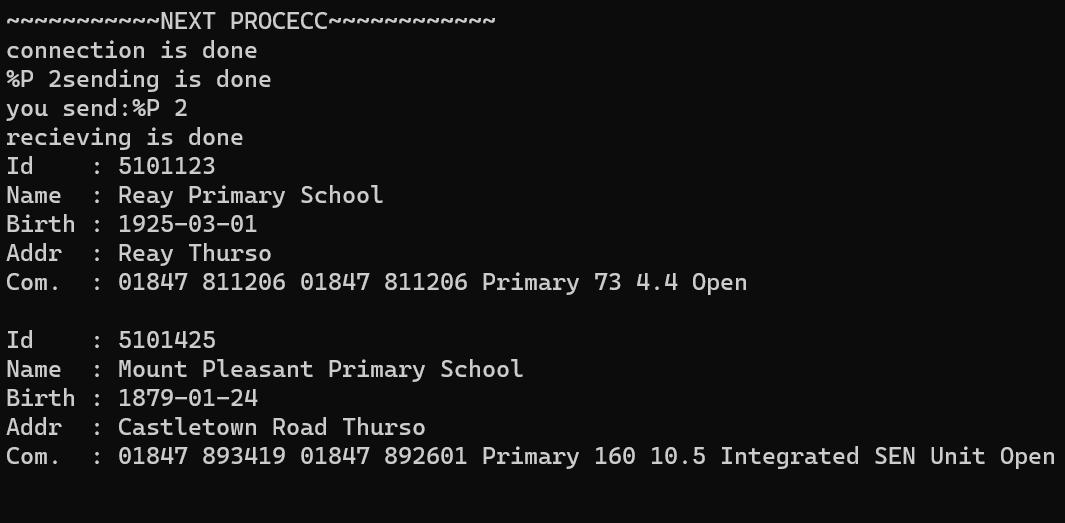
\includegraphics[width=10cm]{pics/p2.png}
\caption{2件プロフィールを表示したときの動作}
\label{fig:p2}\vspace{0zh}
\end{figure}
\begin{figure}[h]
\centering
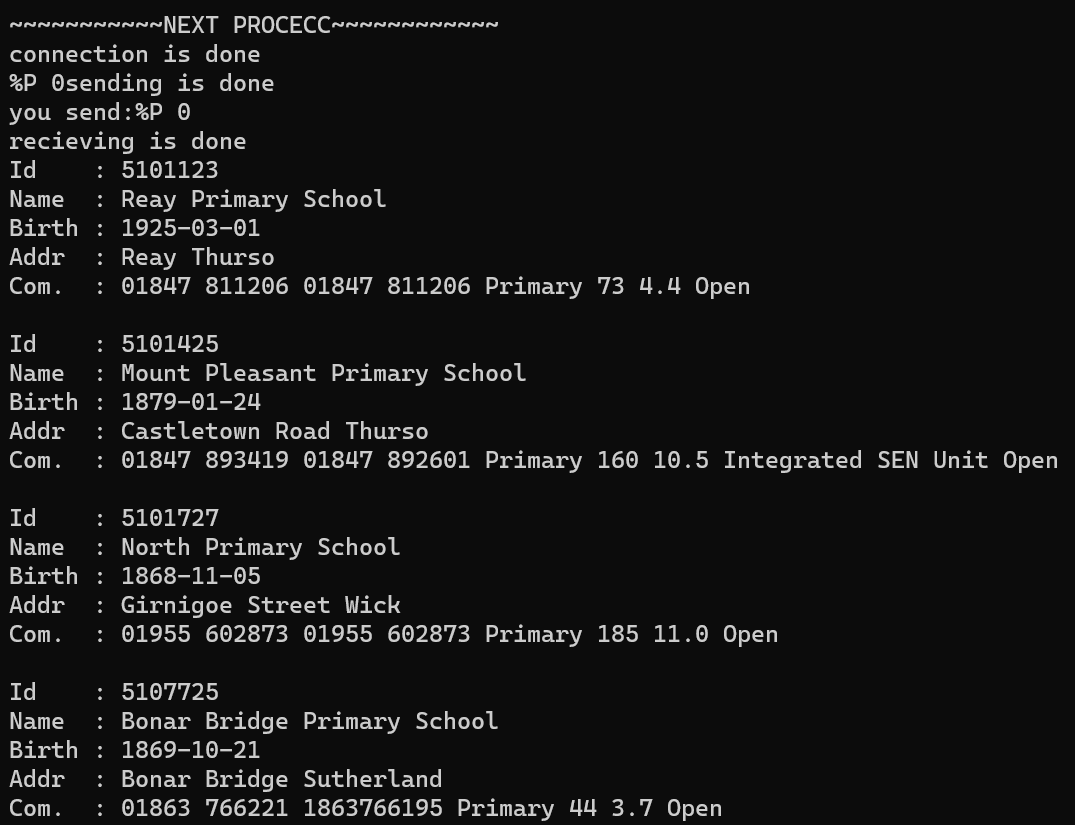
\includegraphics[width=10cm]{pics/p0.png}
\caption{登録してある全件を表示した時の動作}
\label{fig:p0}\vspace{0zh}
\end{figure}

前提として,コマンドを入力するタイミングで4件プロフィールを登録してある.図\ref{fig:p2}より,\%P 2と入力すると2件分のプロフィールを受信していることがわかる.\%P 0は全件表示するコマンドで,動作例の図\ref{fig:p0}より登録してあるプロフィール4件全て表示されていることがわかる.
\subsection{\%R}
\%Rはサーバー側でsvc形式のファイルを読み込みするコマンドである.クライアント側でファイル読み込みする前のプロフィール件数と,読み込んだ後のプロフィール件数を表示し,動作を確認する.なお,読み込む前は4件プロフィールを登録しており,読み込むファイルには121件プロフィールが書き込まれている.読み込む前のプロフィール件数を図\ref{fig:r},ファイルを読み込んだ後のプロフィール件数を図\ref{fig:r121}に示す.
\begin{figure}[h]
\centering
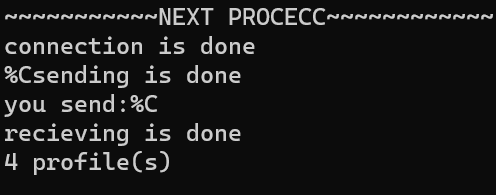
\includegraphics[width=10cm]{pics/R4.png}
\caption{読み込む前のプロフィール件数}
\label{fig:r}\vspace{0zh}
\end{figure}
\begin{figure}[h]
\centering
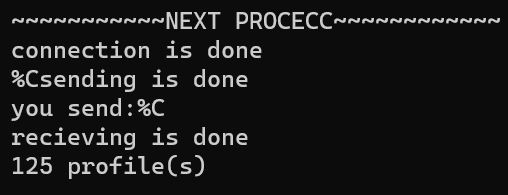
\includegraphics[width=10cm]{pics/R121.png}
\caption{ファイルを読み込んだ後のプロフィール件数}
\label{fig:r121}\vspace{0zh}
\end{figure}

図\ref{fig:r}では既に登録されてある4件のプロフィール件数が表示されている.対して,図\ref{fig:r121}では4件のプロフィールに加えて,121件新たにプロフィールを読み込んだことから125件プロフィールが登録されていることがわかる.\%Rコマンドは正しく動作しているといえる.
\section{プログラムの作成過程に関する考察}
\%P 0で全件を表示しようとするとき,100から200程度のプロフィール件数であれば問題なく表示することができた.しかし1000件程度になるとバッファサイズが足りずサーバー側でSegmentation Faultが発生した.この問題に対して,バッファサイズを100万にし,メモリに余裕を持たせることで解決した.
しかし,常に100万バイトメモリを確保してあることは効率がわるいため,改善案としてmalloc関数を用いて最低限のバッファサイズに加えて,件数表示に必要なバッファサイズを動的に確保することで負荷の少ないプログラムになる.
\section{得られた結果に関する考察}
コマンド\%Pで登録されているプロフィールを表示することができる.この機能を応用して,サーバー側から送られてきたプロフィールに関するバッファをクライアント側で標準出力することでサーバー側のファイルをクライアント側に転送する技術が実現できる.


\end{document}
